\subsection{Specific Applications}
\label{subsec:03_applications}

In this section we take a closer look at applications that are linked to cybersecurity on a secondary level: Here the Blockchain is not per se used to mitigate direct cybersecurity threats, but is used to make applications more robust, error-prone and less vulnerable. 

\subsubsection{Assessment Criteria}
Below we want to introduce different scenarios of applications (implemented or proof-of-work drafts) for the Blockchain technology and apart from a brief introduction of the challenges and problems of this specific field, answer the following questions:
\begin{enumerate}
	\item What is the quality of this specific type of application regarding cybersecurity? 
	\item How does the application make use of the Blockchain Technology?
	\item Is the Blockchain really needed or could the problems be solved without it? 
\end{enumerate}
To answer question number 3 we are going to make use of the below schema presented by \citeauthor{Wust2017}, that helps deciding when the use a blockchain, what kind of blockchain and when a use is not necessary.
\begin{figure}[ht!]
  \begin{center}
  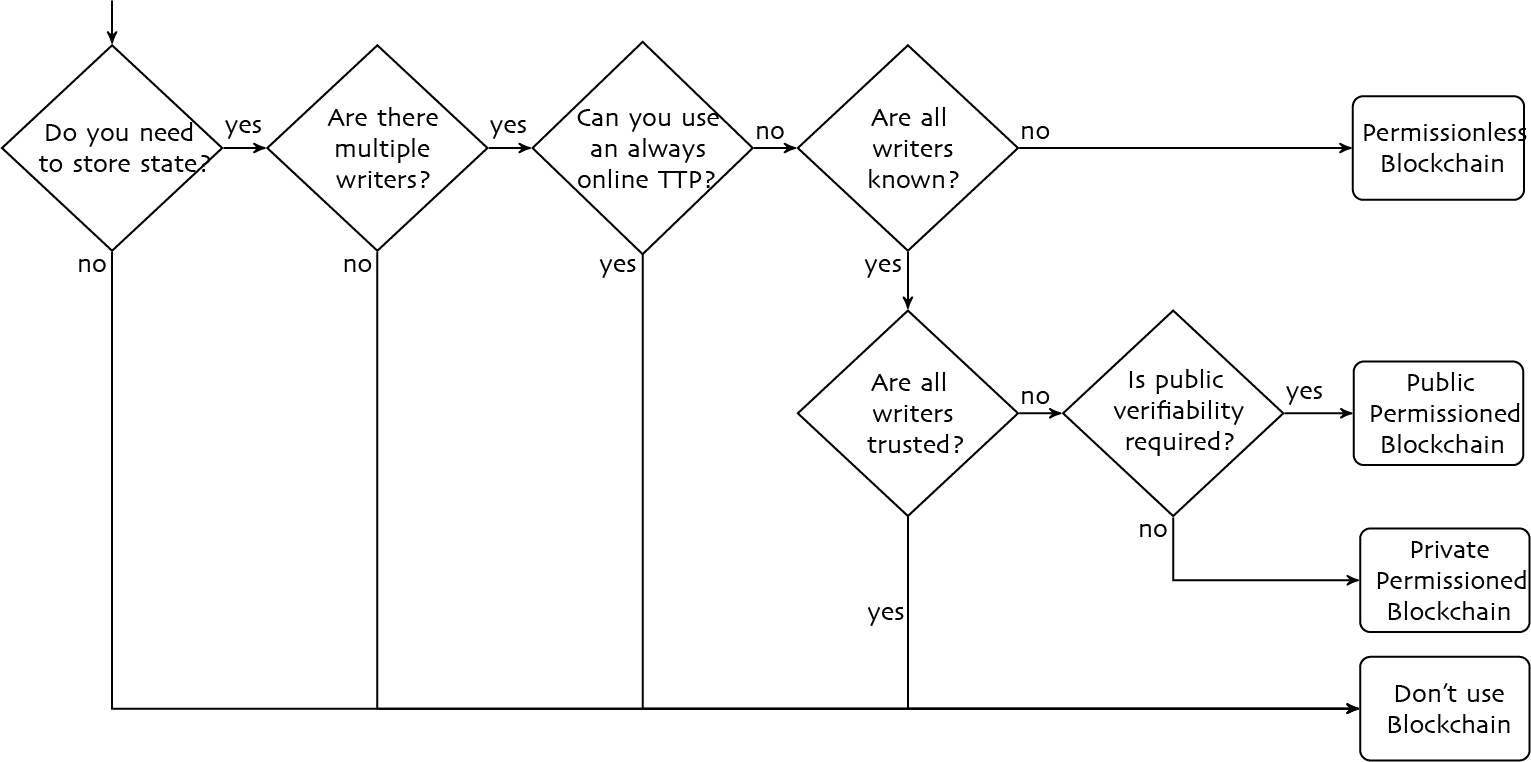
\includegraphics[scale=0.6]{Talk7/img/app/BCorNot}
 	\end{center}
  \caption{Do you need a Blockchain?}
 	\label{blockchain_or_not}
\end{figure}

\subsubsection{E-Voting}
The ability to vote, is the very foundation of every successful democracy and must be accessible for all eligible citicens. Most common systems today are paper-based voting systems, have two major drawbacks.
\begin{enumerate}
	\item They do not scale very well
	\item They rely on the procedural security of officials conducting their jobs.
\end{enumerate}}

And while various e-Voting systems exist, they all come with multiple security vulnerabilities, that lead to an enourmous risks of election rigging and fraud. 
The Blockchain on the other hand offers a transparent and incorruptible database that cannot have a single point of failure or be controlled by a single entity. It therefore immediately comes to mind when facing the above stated problems. Meanwhile new questions of privacy and authenticating the writers arise.

Several systems exist up till today that make use of the blockchain technology. They all differ regarding to the amount of integration and the role of the Blockchain. Different use cases either in theory or in practice have already been tested on smaller county elections or within private organizations. A quite exhaustive overview can be found in \cite{BenAyed2017}. According to \citeauthor{BenAyed2017} these system had the general problem, that single points of failure still existed and that critical parts of the code where closed.
Most existing systems such as Votebook(Source) or Vote Watchers(Source) still dont fully integrate the blockchain but rather use it as underlying database system in the form of a private permissioned blockchain. Those systems still rely on paper ballots. In this case people have to authenticate by showing up in real life at a real world voting booth, that uses the Blockchain for its tamper-proofness, its ability to account as an auditing system and because each voting booths results can be aggregated with all other stations to generate a final result in the end.
According to \citeauthor{Osgood2016} these systems follow the only doable approach, as it doesnt deny the fact, that voters have to identify somewhere
Follow my Vote (Source) follows a fundamentally different approach, because it actually fully integrated the blockchains ability to act as a distributed ledger. Each voter installs a local "Voting Box" on his computer, authenticating via uploaded official documents through the organization that holds the election. Each voter requests ballot online and votes. Nevertheless, according to \citeauthor{Osgood2016} this idea is fundamentally flawed as authentication mechanisms are still an issue and the technique could scare off remote voters.

Within all these systems, two fundamental questions seem to remain unanswered:
\begin{enumerate}
	\item \textbf{Authenticating users and the existence of a trusted third party}:	The riters of the blockchain are either directly or undirectly the voters themselves. To authenticate them, an organization that has all the data about them, is necessary. In most cases this leaves only the government as option. But according to the diagram by  \citeauthor{Wust2017} the use of Blockchain technology only makes sense if no thrusted third party exists. Therefore, it is the role of the government that causes the dilemma itself. If the non-existing trust in the government is the justification for the use of the Blockchain, the question arises whether the government can be trusted regarding the authentication of the voters. Even though a systematic rigging is harder to achieve with this approach, the problem remains at hand. 
	\item \textbf{The user as single point of failure}: While the Blockchain does seem to be perfect for a voting situations, its justification remains questionable. Especially, because it still leaves the most important point of failure unprotected: The user himself. Even the most tamperproofed, blockchain-based voting system does not prevent hackers from a man-in-the-middle attack from a compromised end-device. 
\end{enumerate}

Many of the desired e-Voting properties that the Blockchain technology provides have trade-offs. The aspect of how much privacy is is granted to the voter, is just one of many. On the other hand, no system has yet been proposed that has been shown to be secure, verifiable and private at the same time. The question of authentifiation comes into play as additional point of failure of the concept.
Therefore, if a online trusted third party exists, the use of the blockchain is not necessary. If the government is trusted as far as the authentification of the voters goes, a public permissioned Blockchain can be a good fit. However the security of the system then relies on the interity of the validators. 
If the government is trusted not at all, there exists no solution that overcomes that systematic flaw in a countries governance.

The Blockchain can therefore be a solution if the question of authentification can be answered satisfactorily. Otherwise a traditional paper based voting system is as good as any voting system including Blockchain based systems or systems that base on a trusted third party.

\subsubsection{Autonomous Vehicles, Smart Cities \& IoT}
Smart vehicles are increasingly connected to infrastructure via the Internet, thus making them part of the IoT. This developement brings obvious advantages, but also many challenges, especially in the area of cybersecurity. Malicious attacks on a vehicle endanger not only the vehicles data and the passengers of the vehicle itself, but also other road users. And while many conventional security and privacy methods exist to reduce the risk of an attack they tend to be ineffective due to centralization, unscalability and unsecure communication architectures \cite{DorriSteger2017}.
Meanwhile the challenges on a secure and yet scalable system for connecting self-driving vehicles with other infrastructure are many: They need to be scalable, secure and tamper-proof, private but at the same time accessible to specific entities, such as traffic management systems or an insurance.

The Blockchain offers solutions by design to many of the before mentioned problems. Therefore various approaches exist to connect self-driving vehicles with a blockchain-based architecture.

\citeauthor{DorriSteger2017}, propose a decentralized privacy-preserving and secure blockchain-based architecture for the smart vehicle ecosystem. It bases on its own Blockchain (Lightweight Scalable Blockchain) that minimizes the overhead and increases scalablility as well as the throughput. 
It consists of clusters of nodes which are connected to the system via Overlay Block Managers (OBMs).  All Transactions are broadcast to and verified by the OBMs. Each vehicle is connected to an overlay consisting of various OBMs that form the nodes of the Blockchain based system.
To ensure the users privacy, each vehicle is equipped with an internal vehicle storage to store sensitive data. It is the vehicle owner himself then, who defines which data is provided to third parties and which data is not.
To make certain Public Keys identifiable in the real world a trusted third party is involved and a centralized mechanism is used. This is needed in the case of service centers and software providers.
Many standard applications such as remote software updates, vehicle insurance, Smart Charging and Vehicle Sharing Devices can be made possible through the use of the ecosystem.

Another approach is presented by \citeauthor{Rowan2017}: Their paper focusses on the communication between two road members through side-channels such as visible light and acoustic signals. To solve the problem of the limited data throughput while trying to securely validate the other communication partner, centralized approaches were discarded due to the high number of manufacturers and standards. Instead a blockchain based domain name system is proposed. This way of exchanging identity information was chosen as most promising way of storing public keys due to its robustness and security regarding large scale attacks.

The communication when two e.g. vehicles meet each other needs to be extremeley fast and include as little overhead as possible and work in the absence of any wireless or any cantralized infrastructure. To make this possible, the handshake, that authenticates the involved partners and establishes a secure session, makes use of the Blockchain in the form of a decentralized Domain Name Service.
In this case the Blockchain is used as a way to replace the need for a central authority when authenticating another vehicle. By creating a decentralized Name Service that binds the licence plate value and an identity together with a certificate it is able to create a good base for a secure session between two verifiably trusted vehicles.

\citeauthor{Sharma2017} proposes a hierarchical system. At the top there exist two trusted third parties that register the vehicles (e.g. Department of Motor Vehicles) and that categorize the vehicles into miner nodes and ordinary nodes (Revocation Authority). Both parties exchange information with each other and the blockchain network consisting of the controller nodes. The controller nodes form the blockchain overlay at the top as they hold the information of the vehicle network and share it in a distributed manner with other controller nodes.
The next layer of the blockchain overlay is made by the miner nodes. Miner nodes are chosen vehicles that store data generated by sensors and applications. The top network supports the sharing of information between members of the blockchain network and is allowed to make specific data requests to the miner nodes, to gather informations from sensors etc.

The approach presented by \citeauthor{Sharma2017} is the only approach so far, that thinks far beyond the incorporation of the blockchain into autonomous vehicles: It presents a framework for the controlled and secured interaction between all kinds of IoT devices. Cars as a special case, are just one of them. The approach is very generally described and the exact mechanisms that include the blockchain are not yet beyond an explanatory stage.
The idea though of having multiple layers of nodes that all incorporate the blockchain, but have different rights to access it, seems very promising and suits well to the hierarchical strucutures that are necessary to organize a smart city network. In some way it can be thought of a system of checks and balances where some nodes have more rights, but their actions can always be seen and verified from everywhere at any time.
Again though, even though the Blockchain is presented as central agent, various central authorities remain necessary if the digital has to be linked with the real world.


Applying the flow-chart by \citeauthor{Wust2017} we run into the same problems as before. The main issue is whether a trusted third party exists and what its role is. Whether it exists explicitely such as in the systems of \cite{Sharma2017} or implicetly such as in the case of \cite{Rowan2017} or \cite{DorriSteger2017}, we always have a third party that comes into play. Whether it is trusted or not is another matter.
Having a trusted third party in play can only need to two different outcomes: Either, the use of the blockchain is not necessary, or a private permissioned blockchain should be chosen \cite{Wust2017}.
The only real advantage the blockchain offers in this case,is its tamperproofness and its transparency. Hence all advantages it offers, are the advantages of a decentral database system.

The idea to run an smart city IoT network on the blockchain suggests itself. 
But by looking at the problems that a IoT network for autonomous vehicles faces we can not identify a single problem that would make the use of the blockchain absolutely necessary. Forcing the blockchain onto such problems leads always to the same result: A private permissioned blockchain that is striped off its real (decentral) powers in order to be controllable and easy to use. Therefore it is nothing else than another form of database, that could be replaced with any other database architecture.




\subsubsection{Personal Data Protection and Sharing in the medical sector}
No specific field is that much torn between data sharing and data protection like the medical sector. One one hand, sharing private data is necessary so ensure safe medication and even save lifes, on the other hand the data is extremely sensitive and can inflict big problems on individuals if made public. 

In the health-care sector three traditional models exist to deal with the facility of interoperability of medical data \cite{Kshetri2017}:
\begin{itemize}
	\item Push model: Medical information is sent from one provider to another
	\item Pull model: A provider asks another provider for information
	\item View model: A provider looks at another providers record.
\end{itemize}
A major drawback to all of these models is that the data is not audited or tracked in a standardized way. For example, if a patient is transferred to a different hospital, the new hospital may not be able to access data that was not "pushed". This lack of audit trail means that there is no guarantee of data integrity from the point where data is generated to the point where it is used. 
It is argued by \cite{Kshetri2017} that the blockchain offers a fourth model, which makes it possible to share medical records securely accross providers during the lifetime of a patient without having the need to include a trusted third party into the process. It leaves the data owner in full control about what is shared and leaves a varifiably audit trail of the data behind.

The combination of IoT and the Blockchain in the healthcare sector is particularly powerfull. With the use of smart contracts, IoT devices carry out autonomous transactions on the Blockchain, while guaranteeing access control and data validity at the same time. Based on these thoughts various products and concepts have been created to make use of the Blockchain.




MedRec by \citeauthor{Azaria2016}:
The MedRec system is a sophisticated network to share and protect clinical data using the blockchain and smart contracts. Via smart contracts on an Ethereum blockchain they log patient-provider relationships that associate a medical record with viewing permissions and data retrieval instructions of execution on external databases.
Providers can add new records associated with a particular patient and patients can atuhorize sharing of records between providers. The involved parties are notified by automated notifications when changes occur or new data is added.
By carrying out different kinds of policies, designed to implement any kind of rules, are carried out by the particular smart contracts to enforce data alteration only by legitimate transactions.
To make the potentially large amount of record representations possible the system provides three different types of smart contracts: 
\begin{itemize}
	\item Registrar Contracts, that map participant identification strings to their Ethereum address identiy, such that the registration of new identities can be restricted to certified institutions.
	\item Patient-PRovider Relationship Contracts: Issued when one node stores and manages medical records of the other.
	\item Summary Contracts, that function as bread crumb trail for participants in the system to locate their medical record history
\end{itemize}

The system consists on system nodes that are run by providers, that require a full server and database infrastructure, and patient nodes that can be run on any mobile device or via a web-interface, using only a local database with the patients own data.
MedRec offers two kinds of incentives to run a system node:
The first one is based on Ethereums own inherent incentivizing model. Miners who managa to solve the crypto-puzzle and to incorporate a block into the chain get an amount of Ether on their account, that allows them to pay for transactions.
The second one is targeting researchers, that get rewarded by getting access to anonymized health data.

An uncovered topic in the whole medical sector that is never mentioned by any of the papers is the right to forget, as granted by e.g. the GDPR. This fundamental right of a person/patient to make records disappear is a big problem once a record is in the blockchain. Of course really letting a medical record disappear in traditional systems might be considered impossible as well, but at least from a theoretical point of view, a traditional system allows the deletion of a record. Meanwhile a blockchain based system, does per design not make it possible to delete anything at all, as it is stored within the chain, in an unmodifiable way.

\citeauthor{Cao2019} propose a different model for dealing with patient data:
Existing cloud solutions for medical records as appealing as they are, have many critical privacy and security concerns, as the records in no case should be leaked. However existing cloud service providers would not accept liability for privacy protection against adversaries and only protect the privacy as much as possible. Additionally, the real location of the records is unclear when using cloud based systems 
\citeauthor{Cao2019} analyze multiple existing cloud-assisted eHealth systems and point out, that existing schemes cannot ensure the correctness and integrity of oursourced medical records. Especially not in the case, when a authorized doctor colludes with the cloud server to modify outsourced records which are generated by him himself.

To answer these problems \citeauthor{Cao2019} propose a secure cloud-based system, that ensures the confidentiality, correctness and integriy of oursourced medical records without introducing any trusted third party. In that system records generated by one doctor during a treatment period, are integrated into a transaction of blockchain-based currencies. Meanwhile the system employs a user-friendly password-based key agreement to establish secure channels between patients and doctors.

The proposed system works in the following way: Each patient makes an appointment with the hospital and obtains a treatment key for diagnosis. With the treatment key, a secure channel between patient and hospital and the doctors is established. 
Before the treatment time, the patient generates warrants to delegate to doctors, that indicate the identities of the treating doctors for a specific treatment time and other auxiliary information.
During the treatment time, doctors generate medical records for the patient: In the single-doctor use-case, these are generated by just one doctor, in the multi-doctor use-case, medical records are successively generated by all treating doctors based on the record by the previous doctor. In the latter case each doctor is not only responsible for his own data, but also for the records his predecessors have generated.
The security of this system relies on the security of the Ethereum blockchain and the secure session established based on the treatment key. It mainly ensures that no malicious doctor can modify any record in an unauthorized or misusing way, due to the timeliness and tamperproofness of the Blockchain.

The system is claimed to be secure against:
\begin{itemize}
	\item medical record modification attacks
	\item imporsonation attacks
	\item change of timeline
\end{itemize}
All mechanisms that ensure the systems security are based on the blockchain. The system therefore is very much dependent on the blockchains mechanisms.

Even though this approach is far less extensive than the MedRec approach it does ensure the secure dealing of medical records through patients and doctors and provides to mechanisms to prevent any forging or tampering with the data through authenticated or unauthenticated people.
The only critical point, that challenges the use of the blockchain is again the question "Are all writers trusted?"\cite{Wust2017}. And again we face the problem, that it is the transitioning part of the whole process, the moment when the real world gets projected by a human being onto the digital world, that imposes the vulnerability.
If we do not trust the doctors to create rightful medical records, why do we consult them? And if we do trust them, why do we need a mechanism that prevents the doctors from forging medical records?
OF course one might argue, that there is always good and bad doctors, and that such a system provides a good control against elements in e.g. a chain of treating doctors. But from a theoretical point of view, the question remains. And leads to the conclusion, that in the end, we cannot outsource trust to a machine. 
Disregarding of this general problem, the system does provide good security mechanisms against impersonation attacks and forgery that are undoubtely useful and an improvement that is produced by the nature of the blockchain itself.
The question whether such a system must be run on the blockchain can therefore not be answered finally. The Blockchain is used to make the system more secure, Yes, but the blockchain cannot take over the responsibility for human or institutional malevolence.


A slightly different focus is taken by \citeauthor{Baccarini2018}. This paper tackles the problem of IoT medical sensors, that store and transfer data. They propose a private Blockchain based on the Ethereum Blockchain, where smart devices can call smart contracts and write records into the Blockchain.
The whole field of IoT devices also spreads into the direction of so called Wireless Body Area Networks (WBANs). In a WBAN a patient is equipped with one or multiple wearable or implanted medical devices that take real-time measurements of vital indicators, such as heart rate or glucose levels. All devices report to one master device that collects and aggregates the data and offers a user friendly interface. 
It is obvious why especially in this field multiple security concerns arise: Live patient data is a lucrative target for hackers and poses not only a threat to the patients health itself, but also to the privacy of its data.
To address these concerns \citeauthor{Baccarini2018} propose integrating WBAN systems with smart contracts on a consortium-managed blockchain in order to provide a distributed data processing service, that creates an immutable log of the transactions between WBAN devices and the health care providers. This system allows for automatic notifications of health events to medical professionals in real time in a secure manner. 
The proposed system works as follows:  
A patient wears one or multiple health monitor devices prescribed an applied by a doctor. The raw data of all devices gets collected and aggregated on a smart phone or a tablet and is then, together with customized threshold variables, sent to a specific smart contract on the blockchain. The smart contract evaluates the data and issues alerts to both patient and healthcare provider, as well as automated treatment instructions to the actuator nodes, if necessary.
In that way no medical information is stored on the blockchain or in the smart contract. The only record that gets stored is that what kinds of  events occured. The data itself is forwarded to a designated storage database. Meanwhile a new transaction is stored in the blockchain, saying that the data was successfully processed. In the same way, all treatment commands from the smart contract and healthcare provider will be recorded as complete in the blockchain.
To authenticate the data later and to prevent and detect alterations, whether on purpose or accident, the blockchain transactions can be linked to the storage base where the patients medical history lies.
The system is based on a private and consortium-led blockchain,which allows only designated members to read the blocks, execure smart contracts or verify new blocks.
Nodes in this system are different healthcare companies, that are predefined, such that no rogue members can sneak in.
Additionally, due to the systems modular and customizable smart contracts, it is very easy to replace or upgrade old contracts or incoporate new ones.

Compared with traditional systems, the blockchain based system offers higher performance regarding the availability, the immutability, privacy and transparency of the data. All due to the blockchains design. Regarding confidentiality and speed, the proposed system performs worse or equal than traditional systems.
The largest challenge of the system is maintaing security at every individual node. Because the traffic of the master device of the WBAN is routet via the users internet connection, the data is possibly transmissioned over an open channel.  Other challenges are key management on a large scale and the block verification times, when the alert issued by the smart contract takes too long.

This system is fundamentally different from the others in one aspect: The initially generated data is generated by an IoT device and is per se, digital. No translation step happens between the generation and the incorporation of the data.
The use of the blockchain as underlying system therefore makes a lot of sense, as it does not just use the blockchain architecture as a replacement for any kind of database, but - especially in the combination with the smart contract - to a real entity that supports the interconnection of IoT devices with the service provider in a distributed, secure and tamperproof manner. The fact that it does not use the blockchain to actually store data, but only to log the transitions emphasized this aspect.
In our opinion, the system by  \citeauthor{Baccarini2018} is the only approach that has real use for the design of the blockchain, without trying to alter its nature. Also according to \citeauthor{Wust2017} the permissioned private blockchain is the right choice, to create maximum privacy, while at the same time distributing the data securly to the right place at the right time.
The still exsiting security flaws (see above) do not have anything to do with the system as such and are a problematic aspect in almost any other approach as well. They could be fixed with no real change to the systems architecture. 

\subsubsection{Concluding remarks}

The covered topics show a broad use of the blockchain in order to increase a systems security. Most of the time the blockchain is chosen as a way to store data in a tamperproof manner and to be able to verify the integrity of the data. 
Most approaches however, be it for reasons of following the trend or other reasons, do not take the blockchain for what it is, and instead try to create a suitable database system that suits their use-case best. Reducing it to a distributed, tamper-proof database. The result is always a private permissioned blockchain, that has no real solution for the intial problem: The incorporation of the data iselft into the blockchain. The human as first actor and the problems that arise with this fact are neglected.
Promising are use-cases where such a human- or translation-factor does not exist per se. Use-cases that already have that kind of data at hand that suits a blockchain scenario. Such approaches can exploit the advantages and properties of the blockchain technology at its fullest, without twisting it to fit a specific purpose.
Therefore, if the blockchain is able to act as its own entity, that in an "intelligent" way - through the use of e.g. smart contracts - is allowed to do what it can best, namely act on its own, distributing data in a secure and tamperproof way and secure it forever, the approach has a huge potential. 